\documentclass[14pt,dvipdfmx,uplatex]{beamer}
\usetheme{Madrid}
\setbeamertemplate{footline}[page number]{}
\beamertemplatenavigationsymbolsempty
\usepackage{mypresentation}
\usepackage{fvextra}
%\usepackage{lucidabr}
%\AtBeginShipoutFirst{\special{pdf:tounicode EUC-UCS2}}
\usepackage{tikz}
\usepackage{tcolorbox}
\usetikzlibrary{arrows}
\usetikzlibrary{shapes.callouts}
\usetikzlibrary{decorations.pathmorphing}
\usetikzlibrary{positioning}

\usepackage[noalphabet]{pxchfon}
\input{jpncolor}

\setgothicfont{migmix-2p-bold.ttf}
%\setgothicfont{YasashisaBold.ttf}
%\setminchofont{migmix-2p-bold.ttf} % 本文
\mathversion{bold}

\setbeamerfont{title}{size=\HUGE{28}{34},family={\yasagoth}}
\setbeamerfont{frametitle}{size=\HUGE{20}{28},series={\yasagoth}}
\setbeamerfont{frametext}{size=\HUGE{20}{28},series={\yasagoth}}
\setbeamertemplate{frametitle}[default][left]
\usefonttheme{professionalfonts}

\setbeamercolor{background}{bg=white}
\setbeamercolor{author}{fg=black}
\setbeamercolor{date}{fg=black}
\setbeamercolor{title}{fg=white, bg=kachi}
\setbeamercolor{frametitle}{fg=white}
\setbeamercolor{normal text}{fg=black}
\setbeamerfont{normal text}{family=\rmfamily, series=\bfseries}
\setbeamercolor{structure}{fg=black}

\makeatletter
\define@key{beamerframe}{t}[true]{% top
  \beamer@frametopskip=.2cm plus .5\paperheight\relax%
  \beamer@framebottomskip=0pt plus 1fill\relax%
  \beamer@frametopskipautobreak=\beamer@frametopskip\relax%
  \beamer@framebottomskipautobreak=\beamer@framebottomskip\relax%
  \def\beamer@initfirstlineunskip{}%
}
\def\header#1{\vskip.5\baselineskip{\large\sffamily #1}}
\tikzset{
  notice/.style  = { fill=shozyohi, white, 
                     rectangle callout, 
                     rounded corners,
                     callout absolute pointer={#1} }
}
\makeatother

\setlength{\leftmargini}{12pt}
\setlength{\leftmarginii}{12pt}

\edef\0{\string\0}
\DeclareTextCommand{\CarriageReturn}{JY2}{\015}

\title{\Large 冊子本の原稿として\\ Markdownを使う\\ \large{-- \LaTeX{}とPandocによる事例から --}}
\author{\sffamily 鹿野 桂一郎\\
\bfseries ラムダノート株式会社\\
\small\bfseries \email{k16.shikano@lambdanote.com} \\ 
%\twitter{golden\_lucky} 
}
\date{\sffamily\footnotesize 2019年11月14日\\ 於\, 「アンテナハウス株式会社 \\ Markdown+CSS/TeXで冊子本を作ってみた」}

\begin{document}
\fontseries{ub}\selectfont

%{\usebackgroundtemplate{\includegraphics[height=1.1\paperheight]{skyrocket.jpg}}%
\frame{\titlepage}
%}

% LaTeXの知識はいりません。
% マークアップされたテキスト原稿を組版してPDFとして出力する、という活動をやったことがあればOK

\setbeamertemplate{background canvas}[vertical shading][bottom=white,top=kachi!15]
\setbeamercolor{frametitle}{bg=kachi, fg=white}
\setbeamercolor{structure}{fg=kachi}


\begin{frame}[t]{\inhibitglue Markdownとは?}
  \sffamily
    \begin{itemize}
      \item \leavevmode\inhibitglue 「プレーンテキストを整形」する記法 \\
        \begin{itemize}
          \item Markdown $=$ テキストエディター上で何となく見た目を再現できる装飾付きのテキスト\\[3ex]
        \end{itemize} 
      \item そのテキストを「HTMLへ変換」するツール
        \begin{itemize}
          \item Markdown $=$ Free software \\ (オリジナルはBSD系ライセンス)
        \end{itemize}
    \end{itemize}
    
    \vfill

    \vbox{\footnotesize\raggedright
    John Gruberによる定義:\\
    \url{https://daringfireball.net/projects/markdown/}
    }
\end{frame}

\begin{frame}[plain]
  \begin{center}
    \HUGE{24}{28}\color{kachi}\yasagoth
    つまりMarkdownとは、\\
    \leavevmode\inhibitglue 「記法」であり\\ 
    \leavevmode\inhibitglue 「表現への変換ツール」である
  \end{center}
\end{frame}

% このような定義であるからして…

\begin{frame}[plain]
  \begin{center}
    \HUGE{28}{34}\color{kachi}\yasagoth
    Markdownは\\ 実装者の数だけある!
  \end{center}
\end{frame}

\begin{frame}[t]{\inhibitglue 私も実装したことがあります}
  \sffamily
  \begin{itemize}
    \item \TeX によるMarkdown処理系
    \item \TeX{}のマクロ言語で実装されていて、Markdownの記法で書いた\LaTeX{}形式の原稿から、そのままPDFを作れる
  \end{itemize}
  \begin{center}
    \begin{columns}[c]
      \begin{column}{.4\textwidth}
      \includegraphics[width=\textwidth]{figures/mdtex-input.png}
      \end{column}
      \begin{column}{.4\textwidth}
      \includegraphics[width=\textwidth]{figures/mdtex-output.png}
      \end{column}
    \end{columns}
  \end{center}

    \raggedright
    \vbox{
    \href{https://github.com/k16shikano/markdown-tex}{github.com/k16shikano/markdown-tex}
    }

\end{frame}

% LaTeXの説明が必要!

\begin{frame}[t]{\inhibitglue \LaTeX{}とは}
  \sffamily
    \begin{itemize}
      \item \leavevmode\inhibitglue 「プレーンテキストを整形」する記法 \\
        \begin{itemize}
          \item \LaTeX{} $=$ テキストエディター上で文書の見た目を指示できる\\[3ex]
        \end{itemize} 
      \item そのテキストを「PDFへ変換」するツール
        \begin{itemize}
          \item \LaTeX{} $=$ Free software (LPPLライセンス)
        \end{itemize}
    \end{itemize}
    \vfill

    \begin{center}\footnotesize\sffamily
    Markdownの定義と同じ!
    \end{center}
\end{frame}

\begin{frame}[plain]
  \begin{center}
    \HUGE{24}{28}\color{kachi}\yasagoth
    つまり\LaTeX{}は、\\
    \leavevmode\inhibitglue 「記法」であり\\ 
    \leavevmode\inhibitglue 「表現への変換ツール」である
  \end{center}
\end{frame}

\begin{frame}[plain]
  \begin{center}
    \HUGE{24}{28}\color{kachi}\yasagoth
    \LaTeX{}とMarkdownは、\\
    どちらも
    \leavevmode\inhibitglue 「記法」であり\\ 
    \leavevmode\inhibitglue 「表現への変換ツール」である
  \end{center}
    \vfill

    \begin{center}\footnotesize\sffamily
      (構造化文章のことは忘れましょう)
    \end{center}
\end{frame}

\setbeamertemplate{background canvas}[vertical shading][bottom=white,top=miru!15]
\setbeamercolor{frametitle}{bg=miru, fg=white}
\setbeamercolor{structure}{fg=miru}

\begin{frame}[plain]
  \begin{center}
    \HUGE{24}{28}\color{kachi}\yasagoth
\LaTeX{}ではPDFを作れるので、\\
Markdownの記法を\\ 
\LaTeX{}に変換さえすれば、\\
PDFが作れる?
  \end{center}
    \vfill

    \begin{center}\footnotesize\sffamily
      (Markdownから\LaTeX{}への変換に対する動機)
    \end{center}
\end{frame}

{\usebackgroundtemplate{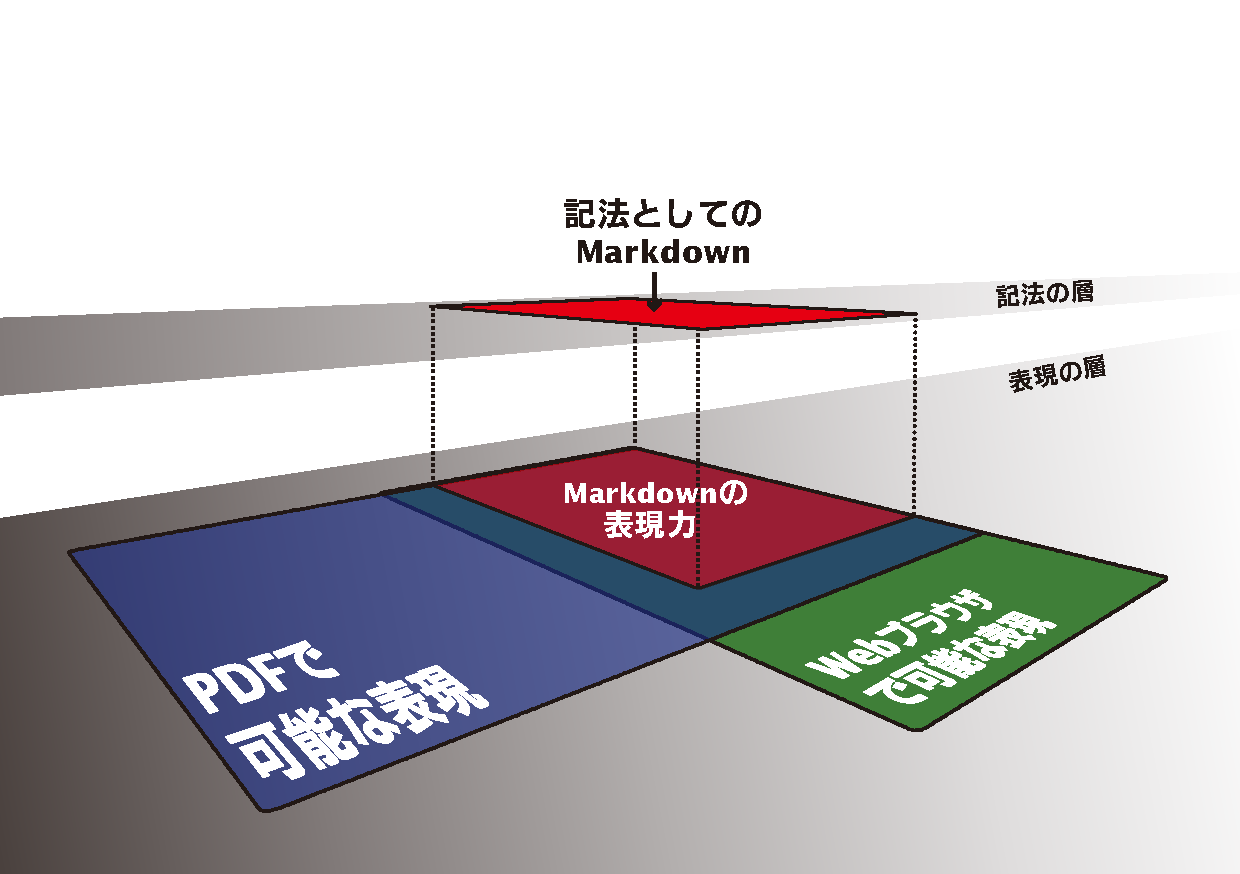
\includegraphics[height=0.95\paperheight]{figures/syntax-rep.pdf}}%
\begin{frame}[t]{\inhibitglue Markdownの表現力}
  \sffamily
  \begin{center}
  \end{center}
\end{frame}
}

{\usebackgroundtemplate{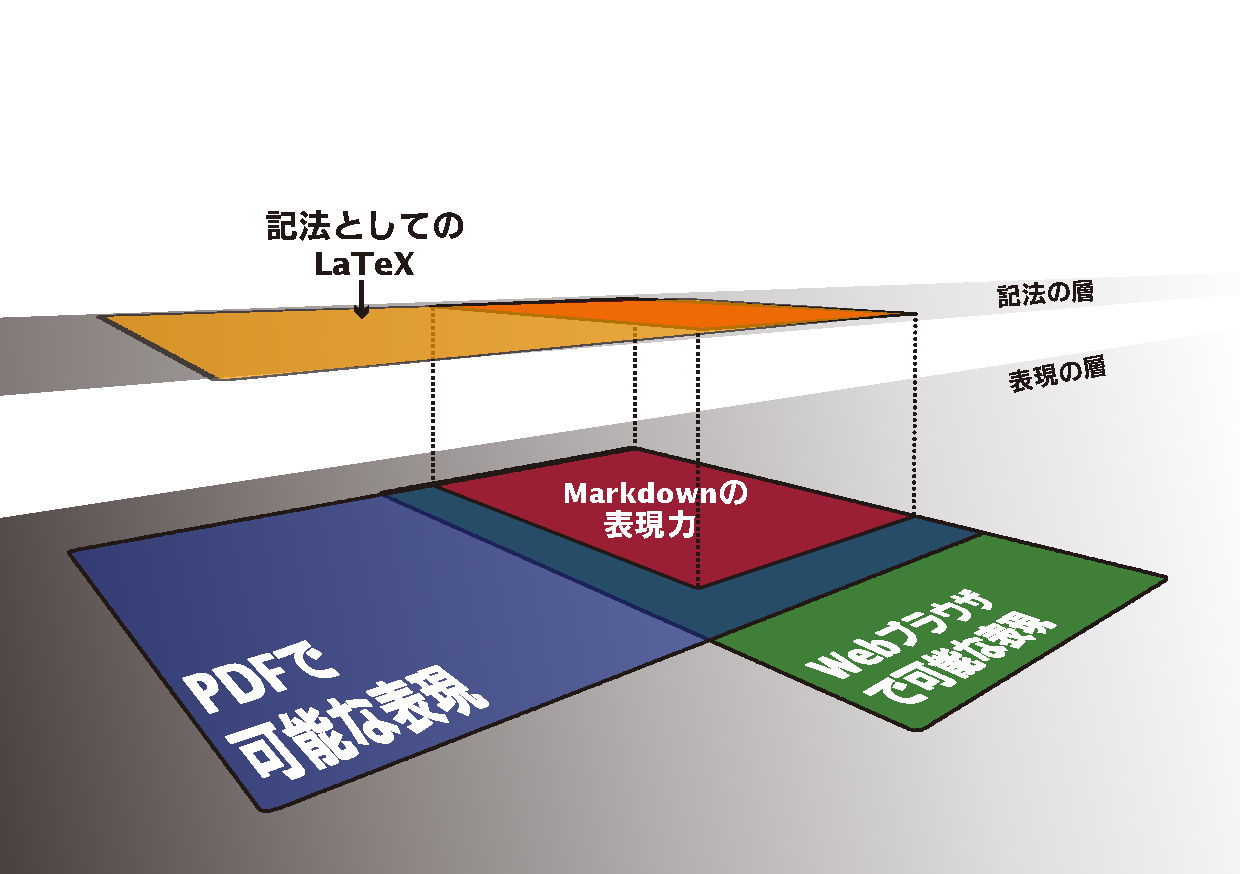
\includegraphics[height=0.95\paperheight]{figures/latexassyntax.pdf}}%
\begin{frame}[t]{\inhibitglue \LaTeX{}の表現力}
  \sffamily
  \begin{center}
  \end{center}
\end{frame}
}

{\usebackgroundtemplate{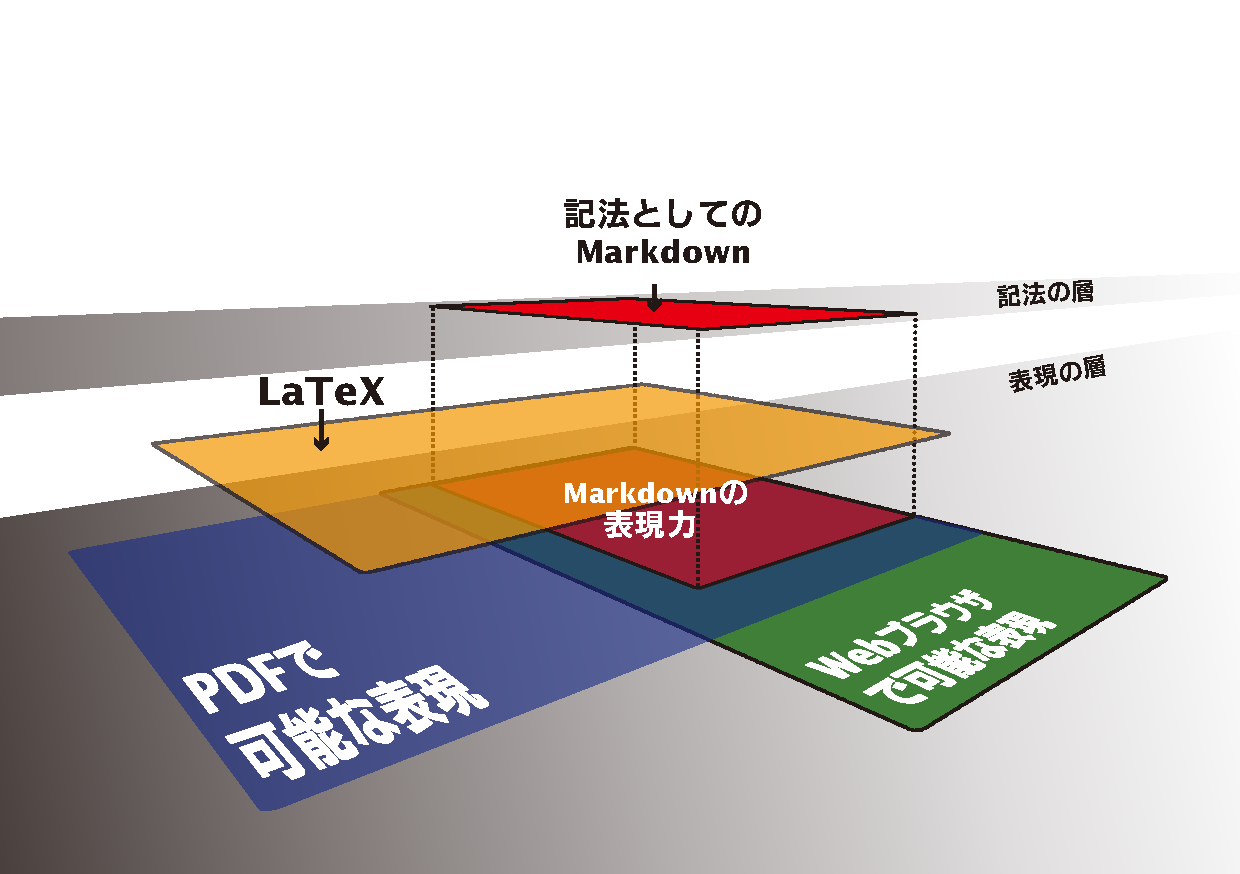
\includegraphics[height=0.95\paperheight]{figures/latexasintermediate.pdf}}%
\begin{frame}[t]{\inhibitglue \LaTeX{}を中間層とすることで\\[-0.5ex] MarkdownからPDFの表現力を得る\\[-.7\baselineskip]}
  \sffamily
  \begin{center}
  \end{center}
\end{frame}
}

\begin{frame}[t]{\inhibitglue Markdownと\LaTeX{}の関係}
  \sffamily
    \begin{itemize}
      \item Markdown $=$\\ \LaTeX{}の標準的な記法の代わりとなる、より簡易な記法\\[3ex]
      \item \LaTeX{} $=$\\ Markdown記法のテキストからHTMLではなくPDFを出力したいときのバックグラウンド
    \end{itemize}

    \vfill

    \vbox{\footnotesize\raggedright
      MarkdownとHTMLの間の関係と、ほぼ同じ関係が成り立っている。
    }
\end{frame}

% 

\setbeamertemplate{background canvas}[vertical shading][bottom=white,top=yamabuki!15]
\setbeamercolor{frametitle}{bg=yamabuki, fg=black}
\setbeamercolor{structure}{fg=yamabuki}

\begin{frame}[plain]
  \begin{center}
    \HUGE{24}{28}\color{black}\yasagoth
MarkdownからPDFを作れる\\
$\neq$ \\
Markdownから冊子本を作れる
  \end{center}
\end{frame}

\begin{frame}[plain]
  \begin{center}
    \HUGE{24}{28}\color{black}\yasagoth
Markdownの表現力では不足\\ する点を\LaTeX{}で直接補えば、\\ 冊子本のPDFを作れるか?
  \end{center}
\end{frame}

\begin{frame}[t]{\inhibitglue \LaTeX{}の一部にMarkdownを使う方法}
  \sffamily
  \begin{itemize}
    \item \leavevmode\inhibitglue 「冊子本のためのPDF」に必要とされる構造だけならば、その選択肢もありえた
    \item 原稿に\LaTeX{}の記法が混在することをどこまで許容できるか
    \item 電子版との原稿の分裂の可能性
  \end{itemize}
    \vfill

    \vbox{\footnotesize\raggedright
      「XML原稿の中にMarkdownの島がある」ような原稿もあった(翻訳書)
    }
\end{frame}

\begin{frame}[t]{\inhibitglue そこでPandoc}
  \sffamily
  \begin{itemize}
    \item \url{https://pandoc.org/}
    \item 多様なドキュメント形式の相互変換ツール
    \item MarkdownからPDFへの変換にも対応
    \item PDFを出力する場合のバックグラウンドには\LaTeX{}が採用されている
  \end{itemize}
    \vfill

    \vbox{\footnotesize\raggedright
      ただし、これは一般向けのキャッチ―な説明。
      Pandocの本懐は、多様なドキュメント形式を「Markdownの構造」でとらえるためのツールという点。
    }
\end{frame}


{\usebackgroundtemplate{\includegraphics[height=0.95\paperheight]{figures/nml-flow.pdf}}%
\begin{frame}[t]{\inhibitglue 不定期刊行誌『 $n$月刊ラムダノート』\\[-0.5ex] 制作フロー\\[-.7\baselineskip]}
  \sffamily
  \begin{center}
  \end{center}
\end{frame}
}

\begin{frame}[t]{\inhibitglue Pandocを採用している理由}
  \sffamily
  \begin{itemize}
    \item Pandocが提供する型は、Markdownの記法から自然に決まるドキュメントの構造
    \item その構造の基本的な構成要素は、冊子本にとっても十分\\
    \begin{itemize}
      \item むしろ最低限の構造しかないので、見た目で原稿をごまかせる余地が減る
      \item 参考:ラムダノートの記事執筆スタイルガイド:\\ {\footnotesize\url{https://gist.github.com/LambdaNote/0d33b7d8284a3c99cffd1a5aa83c115f}}
    \end{itemize}
    \item 足りない構造を補う、豊富なツールチェインと拡張性
    \begin{itemize}
      \item 素のMarkdownと親和性の高い「記法」がセットで提供されている(これが最も重要)
    \end{itemize}
  \end{itemize}
\end{frame}

{\usebackgroundtemplate{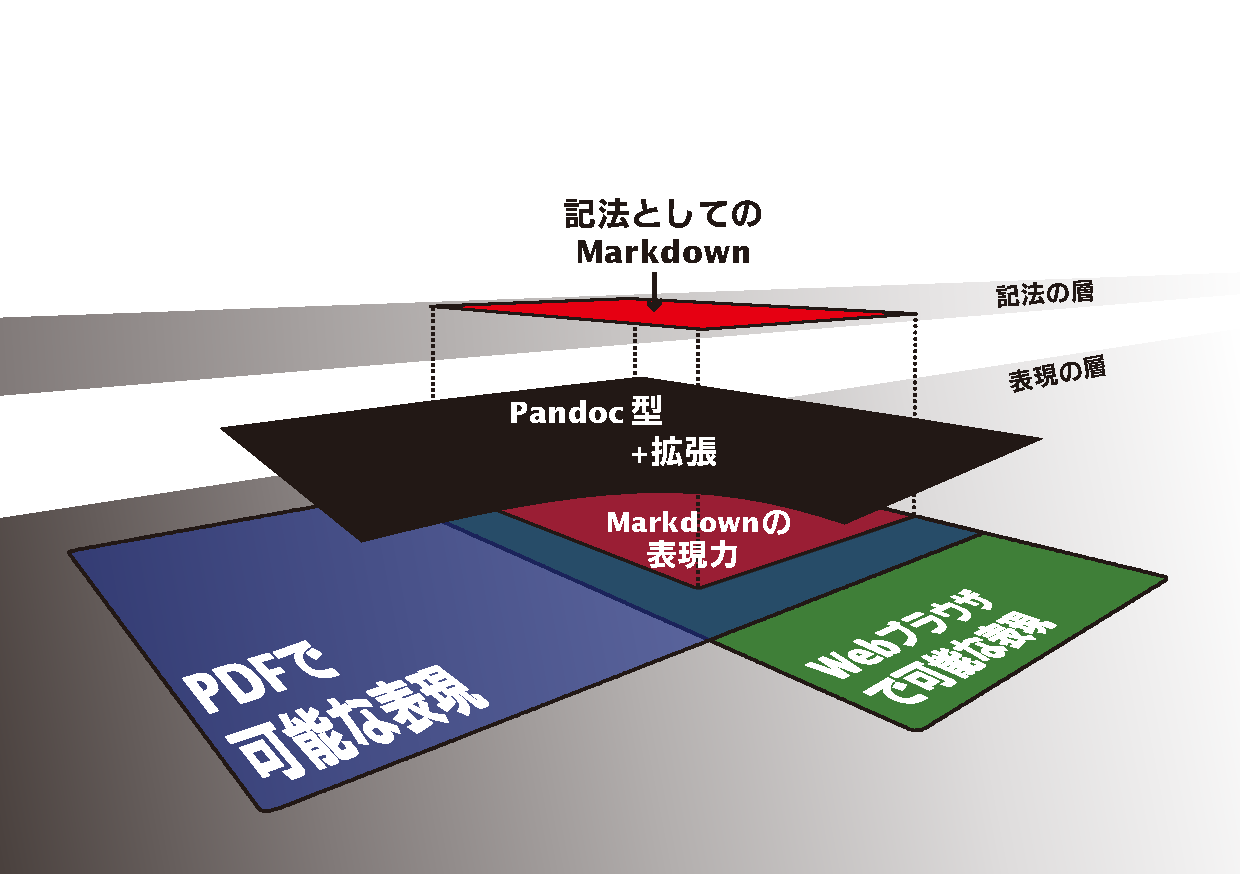
\includegraphics[height=0.95\paperheight]{figures/pandoc.pdf}}%
\begin{frame}[t]{\inhibitglue Pandocを中間層とすることで\\[-0.5ex] Markdownから冊子本の表現力を得る\\[-.7\baselineskip]}
  \sffamily
  \begin{center}
  \end{center}
\end{frame}
}

\begin{frame}[t]{\inhibitglue Pandocが提供する型}
  \sffamily
  \begin{center}
    \begin{columns}[c]
      \begin{column}{.5\textwidth}
      \includegraphics[width=\textwidth]{figures/pandoc-type-block.png}\\
      \hbox{\tiny 出典:\url{http://hackage.haskell.org/package/pandoc-types} }
      \end{column}
      \begin{column}{.3\textwidth}
      \includegraphics[width=\textwidth]{figures/pandoc-type-inline.png}
      \end{column}
    \end{columns}
  \end{center}
\end{frame}

\begin{frame}[t]{\inhibitglue 冊子本で使えるPandocの拡張}
  \sffamily
  \begin{itemize}
    \item YAML Metadata Block
    \item pandoc-citeproc + CSL (参考文献)
    \item \texttt{\{...\}}構文による属性指定 \\
    \begin{itemize}
      \item pandoc-crossref (相互参照)
      \item コードブロックのハイライト
    \end{itemize}
    \item footnotes (脚注)
    \item Pipe Tables (表)
    \item Pandocフィルター
  \end{itemize}
\end{frame}

\begin{frame}[t]{\inhibitglue YAML Metadata Block}
  \sffamily
  \begin{itemize}
    \item 冊子本の構成やタイトルなどの情報を、原稿ファイルにYAML形式で埋め込める
    \item YAMLが記法の一部になっているといえる
  \end{itemize}
  \begin{center}
  \includegraphics[width=.9\textwidth]{figures/yaml-header.png}\\
  \end{center}
\end{frame}

\begin{frame}[t]{\inhibitglue pandoc-citeproc + CSL (参考文献)}
  \sffamily
  \begin{itemize}
    \item Bib\TeX{}形式で保存した参考文献が利用できる
    \item citationの記法は\texttt{[@...]}
    \item citationとエントリの整形には\\ CSL({\footnotesize\url{https://citationstyles.org/}})を利用
  \end{itemize}
  \begin{center}
  \includegraphics[width=.9\textwidth]{figures/citeproc.png}\\
  \end{center}
\end{frame}

\begin{frame}[t]{\inhibitglue pandoc-citeproc + CSL (参考文献)}
  \sffamily
  \begin{itemize}
    \item Bib\TeX{}形式で保存した参考文献が利用できる
    \item citationの記法は\texttt{[@...]}
    \item citationとエントリの整形には\\ CSL({\footnotesize\url{https://citationstyles.org/}})を利用
  \end{itemize}
  \begin{center}
  \includegraphics[width=.9\textwidth]{figures/citeproc2.png}\\
  \end{center}
\end{frame}

\begin{frame}[t]{\inhibitglue pandoc-crossref (相互参照)}
  \sffamily
  \begin{itemize}
    \item 図、表、コードリスト、節などにIDを指定し、本文から番号で参照できるようにする機構
    \item IDの付与には属性の記法\texttt{\{\#...\}}を使う
    \item 参照にはcitationと同じ記法\texttt{[@...]}を使う
    \item \LaTeX{}に任せるべきではない
  \end{itemize}
  \begin{center}
  \includegraphics[width=.9\textwidth]{figures/crossref.png}\\
  \end{center}
\end{frame}

\begin{frame}[t]{\inhibitglue コードブロックのハイライト}
  \sffamily
  \begin{itemize}
    \item コードブロックに属性を指定することで、予約語のハイライトなどを有効にする機構
    \item 属性の記法\texttt{\{...\}}を使う
    \item \LaTeX{}に任せることもできる
  \end{itemize}
  \begin{center}
  \includegraphics[width=.8\textwidth]{figures/code-highlight.png}\\
  \end{center}
\end{frame}

\begin{frame}[t]{\inhibitglue footnotes (脚注)}
  \sffamily
  \begin{itemize}
    \item 脚注のための簡便な記法
    \item \texttt{[\^{}aaa]}および\texttt{[\^{}aaa]: ...}
  \end{itemize}
  \begin{center}
  \includegraphics[width=.9\textwidth]{figures/footnote.png}\\
  \end{center}
\end{frame}

\begin{frame}[t]{\inhibitglue Pipe tables (表)}
  \sffamily
  \begin{itemize}
    \item さまざまな表の記法のうち、表現力と記述性のバランスがよい
    \item 表のレンダリング結果を完全に制御できるわけではない
  \end{itemize}
  \begin{center}
  \includegraphics[width=.9\textwidth]{figures/table.png}\\
  \end{center}
\end{frame}

\begin{frame}[t]{\inhibitglue Pandocフィルター}
  \sffamily
  \begin{itemize}
    \item Pandoc型の値を直接、プログラムにより操作できる
    \item \leavevmode\inhibitglue 「本文内の行コメント」のような仕組みを導入することも可能に
  \end{itemize}
  \begin{center}
  \includegraphics[width=.9\textwidth]{figures/filter.png}\\
  \end{center}
\end{frame}

\begin{frame}[t]{\inhibitglue それでも\LaTeX{}の知識は必要}
  \sffamily
  \begin{itemize}
    \item 冊子本の全体構成を組み立てるには、Pandocのテンプレート機構か、それに類する仕組みが必要になる
    \item \leavevmode\inhibitglue 「最後の追い込み」が必要
    \item エスケープの問題
    \item 数式の記法は?
    \item 索引の記法は?
    \item 生の\LaTeX{}記法を埋め込めるか
    \begin{itemize}
      \item 「構造」ないと埋め込みにくい
      \item MarkdownにHTMLを埋め込めるのは、HTMLが記法であり「構造」でもあるから
    \end{itemize}
  \end{itemize}
\end{frame}

\setbeamertemplate{background canvas}[vertical shading][bottom=white,top=toki!15]
\setbeamercolor{frametitle}{bg=toki, fg=black}
\setbeamercolor{structure}{fg=toki}

\begin{frame}[t]{\inhibitglue まとめ}
  \sffamily
  \begin{itemize}
    \item Markdownはドキュメントの構造というより、むしろ記法
    \item したがってMarkdown原稿から冊子本(のためのPDF)を作る際も、構造にスタイルを当てはめるというXML的な考え方でなく、むしろ構造を暗に表す記法そのものが問題になる
    \item Pandocは、Markdownの記法により決まる構造を利用しやすくすると同時に、Markdown自体に欠けている冊子本で必要となる記法も提供してくれている
  \end{itemize}
\end{frame}

\begin{frame}[t]{\inhibitglue 宣伝}
  \sffamily
  \begin{itemize}
    \item ラムダノート株式会社は出版を中心として技術文書まわりのお手伝いをいろいろする会社です
    \begin{itemize}
      \item \url{https://lambdanote.com}
    \end{itemize}
  \end{itemize}
  \begin{center}
    
\includegraphics[width=.5\textwidth]{figures/main-logo.pdf}
  \end{center}
\end{frame}

{\usebackgroundtemplate{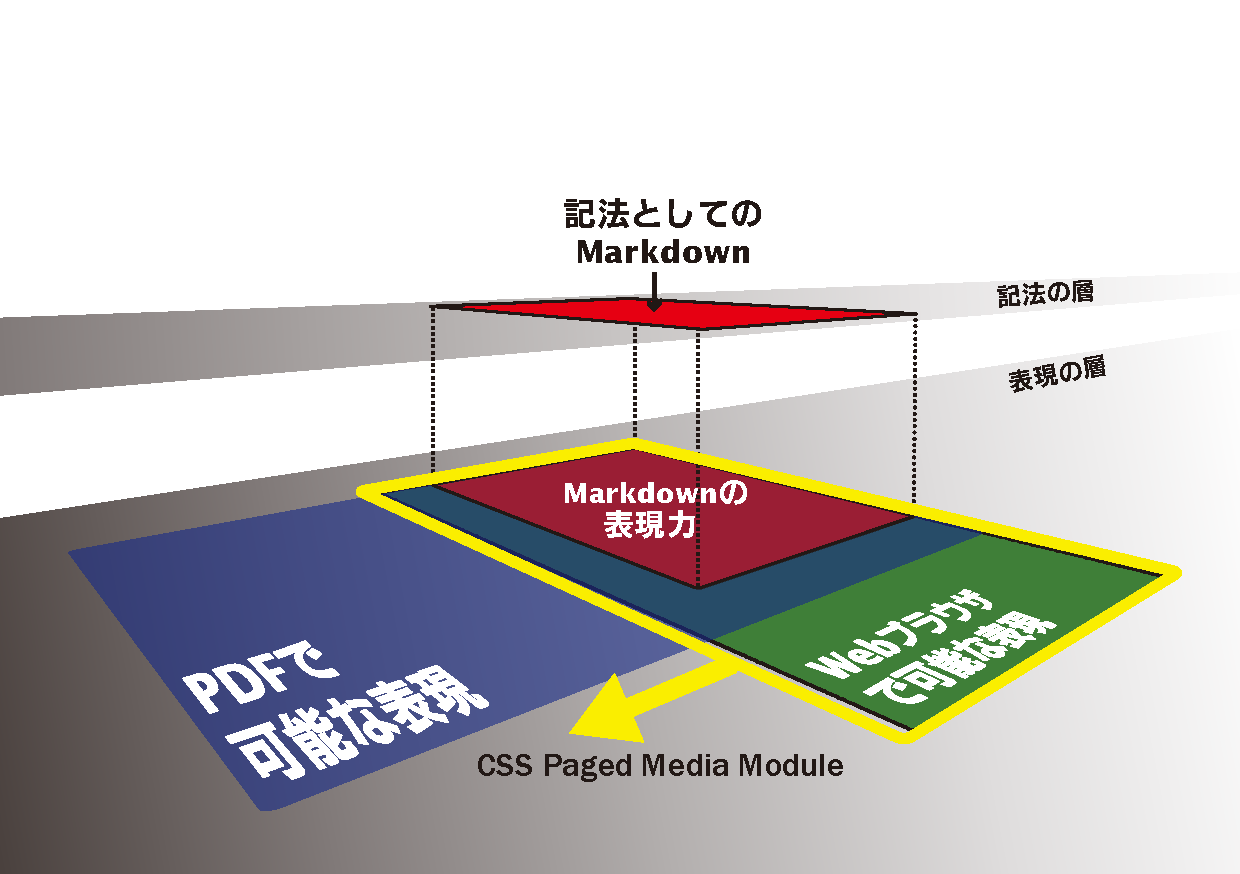
\includegraphics[height=0.95\paperheight]{figures/css.pdf}}%
\begin{frame}[t]{\inhibitglue おまけ:Markdown+CSSの方向性?}
  \sffamily
  \begin{center}
  \end{center}
\end{frame}
}

\end{document}
